\documentclass{article}
\usepackage{csquotes}
\usepackage[spanish]{babel}
\usepackage{graphicx}
\usepackage{float}
\usepackage{amsmath}        % para los vectores columnas
\usepackage{amsfonts}       % para las negrita de pizarra
\usepackage{amssymb}        % para simbolos matematicos
\usepackage{hyperref}       % para utilizar referencias
\usepackage{multirow}       % para las tablas
\usepackage{dsfont}
\usepackage{listings}
\usepackage{xcolor}
\usepackage{ragged2e}
\definecolor{codegreen}{rgb}{0,0.6,0}
\definecolor{codegray}{rgb}{0.5,0.5,0.5}
\definecolor{codepurple}{rgb}{0.58,0,0.82}
\definecolor{backcolour}{rgb}{0.95,0.95,0.92}
\lstdefinestyle{mystyle}{
    backgroundcolor=\color{backcolour},   
    commentstyle=\color{codegreen},
    keywordstyle=\color{magenta},
    numberstyle=\tiny\color{codegray},
    stringstyle=\color{codepurple},
    basicstyle=\ttfamily\footnotesize,
    breakatwhitespace=false,         
    breaklines=true,        
    captionpos=b,                    
    keepspaces=true,                 
    numbers=left,                    
    numbersep=5pt,                  
    showspaces=false,                
    showstringspaces=false,
    showtabs=false,                  
    tabsize=2
}
\lstset{style=mystyle}

\usepackage{enumitem,multicol,setspace}
\newcounter{subenum}[enumi] % para las multicolumnas
\renewcommand{\thesubenum}{\arabic{subenum}}
\usepackage[nomessages]{fp}
\FPeval\thecolwidth{round(1/4:4)}% Specify number of columns -> column width
\newcommand{\newitem}[1]{%
  \refstepcounter{subenum}%
  \parbox{\dimexpr\thecolwidth\linewidth-.5\columnsep}{%
    \makebox[\labelwidth][r]{(\thesubenum)\hspace*{\labelsep}}%
    #1}\hfill%
}

\usepackage{scalerel,stackengine} % para el sombrero
\stackMath
\newcommand\rhat[1]{%
\savestack{\tmpbox}{\stretchto{%
  \scaleto{%
    \scalerel*[\widthof{\ensuremath{#1}}]{\kern-.6pt\bigwedge\kern-.6pt}%
    {\rule[-\textheight/2]{1ex}{\textheight}}%WIDTH-LIMITED BIG WEDGE
  }{\textheight}% 
}{0.5ex}}%
\stackon[1pt]{#1}{\tmpbox}%
}
\parskip 1ex

\usepackage{mathtools}      % floor y ceil
\DeclarePairedDelimiter\ceil{\lceil}{\rceil}
\DeclarePairedDelimiter\floor{\lfloor}{\rfloor} 

\usepackage[style=authoryear-comp]{biblatex}

\title{Título de tu Informe}
\author{Tu Nombre}
\date{\today}
\begin{document}
\maketitle

\justifying{}

\newpage
\section{Consideraciones}

Este documento está pensado para que sirva de guía, e incluso template a la hora de realizar un informe para la materia (por no decir, cualquier documento formal en la facultad). La idea es utilizar \LaTeX, pura y exclusivamente para que tenga un formato acorde. Es decir, no hecho en un simple procesador de texto (como pudiese ser Word). 

Aquí sólo se mostraran algunas de las cosas que se pueden hacer con \LaTeX. Si se quiere hacer algo específico, o de otra forma, abunda la documentación (y artículos de StackOverflow) al respecto. 

Definimos ciertos lineamientos técnicos a considerar para los informes: 
\begin{itemize}
    \item En el informe debe estar incluido el código más importante (es decir, los algoritmos, no un main) cuando corresponda. 
    \item Debe estar explicado cómo se hacen los sets de prueba. Inclusive, si notan alguna falencia con esta generación que pueda afectar de alguna forma el análisis del resultado, se espera que lo enuncien (hay trabajos donde esto no sucederá, pero hay trabajos donde sí, especialmente cuando vemos aproximaciones). 
    \item Los gráficos deben estar bien generados: deben tener título, los ejes deben tener tanto qué refieren como qué unidad de medida usan (en caso de tenerla). En caso de tener gráficos superpuestos, debe quedar claro qué es cada gráfico. 
    \item \textbf{Importante}: en caso de tener que realizar una reentrega (y por ende, tener que cambiar cosas del informe), salvo que haya que rehacer una enorme cantidad del mismo, no modificar el informe anterior sino agregar un anexo al final indicando las correcciones realizadas en la nueva entrega, para agilizar las correcciones. 
\end{itemize}

A su vez, dejamos algunas breves líneas sobre cuestiones de redacción: 
\begin{itemize}
    \item Evitar errores ortográficos y gramaticales. 
    \item El lenguaje debe ser técnico. No tiene que por eso ser un texto aburrido, pero evitar frases como "\textit{la cosa que más me complicó fue...}", "\textit{creo que...}". 
    \item Usar plural de modestia, incluso si el trabajo fuera realizado por una única persona.
\end{itemize}
\newpage
\justifying{
\hypertarget{res}{\section*{Resolución}}
\section{Algoritmo para elegir las monedas}

En este trabajo de ejemplo realizaremos el análisis teórico y empírico de diferentes algoritmos que sirven para resolver el mismo problema: obtener el orden en que se deben elegir las monedas para maximizar la ganancia obtenida de un arreglo de $n$ monedas. 

\subsection{Algoritmo para encontrar el optimo}

El algoritmo plantea una matriz de $n * n$, siendo $n$ la cantidad de monedas, donde para cada coordenada $i$, $j$ de la matriz, encontramos una solucion para un problema de dimensiones $i$, $j$.
Luego se llena las diagonales, donde las corrdenads $i$ y $j$ son iguales, $i = j$, y la diagonal donde la coordenada $j$ es uno mas que la $i$, $i = j + 1$, con los valores de los dos casos base, siendo estos:
\begin{itemize}
    \item tener una sola mondea, donde el optimo es la moneda en si.
    \item tener dos monedas, donde el optimo es la mas grande entre la dos.
\end{itemize}
Luego recorre la parte superior de la matriz (ya que los punteros $i$, $j$ que 
apuntan al principio y final del array de monedas respectivametne, nunca se
intercambian, lo que es igual, se cummple que $i <= j$), llenando cada lugar de la matriz con la solucion del problema de tamaño $i$, $j$.
Es asi que una vez completamos la matriz, encontramos la solucion optima para nuestro problema original en la coordenada $i = 0$ y $j = n$.

Aqui el codigo usado para generar la matriz con los valores optimos para todos los problemas de dimensiones $i$, $j$.

\begin{lstlisting}[language=Python]
def elegir(monedas):
    opt = [[0] * len(monedas) for i in range(len(monedas))]
    
    # Casos base con una moneda
    for i in range(0, len(monedas)):
        opt[i][i] = monedas[i]
        
    # Casos base con 2 monedas
    for i in range(0, len(monedas) - 1):
        j = i + 1
        opt[i][j] = max(monedas[i], monedas[j])
    
    for i in range(len(opt) - 1, -1, -1):
        for j in range(i + 2, len(opt)):
            # Sophia toma la primera
            # Achico mi rango segun lo que eliga Mateo
            opt_i = opt[i + 2][j] if monedas[i + 1] > monedas[j] else opt[i + 1][j - 1]
            
            # Sophia toma la ultima
            # Achico mi rango segun lo que eliga Mateo
            opt_j = opt[i + 1][j - 1] if monedas[i] > monedas[j - 1] else opt[i][j - 2]
            
            opt[i][j] = max(monedas[i] + opt_i, monedas[j] + opt_j)
            
    maxima_ganancia = opt[0][len(opt) - 1]
    sol = solucion(opt, monedas, [], 0, len(opt) - 1)
    return sol
\end{lstlisting}

La forma de obtener nuesta matriz optima es la siguente.
Se plantea que para cada problema de dimensiones $i$, $j$, donde queremos encontrar que moneda elegir para mazimizar la ganancia, la moneda en la posicion $i$ (la primera), y la moneda $j$ (la ultima), se puden analizar las siguentes opciones.

\begin{enumerate}
    \item Sophia toma la primera moneda, la moneda $i$ y Mateo elige la mayor entre las monedas $i + 1$ y $j$.

    \begin{enumerate}
        \item Si mateo eligie la moneda $i + 1$ el rango $(i, j)$ se achica a $(i + 2, j)$, por lo que nuestra solucion sera el valor de la moneda $i$ mas la solucion del rango $(i + 2, j)$.

        $opt(i, j) = moneda_i + opt(i + 2, j)$

        \item Si mateo eligie la moneda j el rango $(i, j)$ se achica a $(i + 1, j - 1)$, por lo que nuestra solucion sera el valor de la moneda $i$ mas la solucion del rango $(i + 1, j - j)$.

        $opt(i, j) = moneda_i + opt(i + 1, j - 1)$

    \end{enumerate}

    \item Sophia toma ahora la ultima moneda, la moneda $j$ y Mateo elige la mayor entre las monedas $i$ y $j - 1$.

    \begin{enumerate}
        \item Si mateo eligio la moneda $i$ el rango $(i, j)$ se achica a $(i + 1, j - 1)$, por lo que nuestra solucion sera el valor de la moneda j mas la solucion del rango $(i + 1, j - 1)$.

        $opt(i, j) = moneda_j + opt(i + 1, j - 1)$

        \item Si mateo eligio la moneda $j$ el rango $(i, j)$ se achica a $(i, j - 2)$, por lo que nuestra solucion sera el valor de la moneda j mas la solucion del rango $(i, j - 2)$.

        $opt(i, j) = moneda_i + opt(i, j - 2)$
    \end{enumerate}
\end{enumerate}

Luego de plantear las cuatro posibles situaciones, podemos ver que, 
sin importar lo que elija sophia, mateo siempre elije la moneda mas grande
por lo que en ambos casos en simplemente realizar una comparacion para ver cual 
es mas grande, segun la situacion de monedas. Esta comparacion determina el rango
de mis soluciones parciales. Luego obtengo mis soluciones parciales para los rangos 
respectivos segun la eleccion de mateo, me quedo con aquella solucion, que maximize mi 
ganancia. 
Entonces Siendo $opt_i$, la solucion para un rango $(i_i, j_i)$, asumiendo que sophia toma la $moneda i$, y, siendo $opt_j$, la solucion para un rango $(i_j, j_j)$, asumiendo que sophia toma la moneda $j$, el optimo para el rango $(i, j)$ queda de la siguente manera.

\[
\text{opt}(i, j) = \max \left( \text{moneda}_i + \text{opt}_i, \; \text{moneda}_j + \text{opt}_j \right)
\]

donde:
\[
\text{moneda}_i + \text{opt}_i = 
\begin{cases} 
\text{monedas}[i] + \text{opt}(i + 2, j) & \text{si } \text{monedas}[i + 1] > \text{monedas}[j] \\[1ex]
\text{monedas}[i] + \text{opt}(i + 1, j - 1) & \text{sino}
\end{cases}
\]

\[
\text{moneda}_j + \text{opt}_j = 
\begin{cases} 
\text{monedas}[j] + \text{opt}(i + 1, j - 1) & \text{si } \text{monedas}[i] > \text{monedas}[j - 1] \\[1ex]
\text{monedas}[j] + \text{opt}(i, j - 2) & \text{sino}
\end{cases}
\]

\subsection{Algoritmo para obtener la reconstruccion de la solucion}

Partiendo de la matriz optima, desarrollamos un algoritmo que brinde la secuencia de monedas que se deberian elegir para obtener la ganancia maxima, mediante llamadas recursivas.

\begin{enumerate}
    \item Casos base.
    \begin{itemize}
        \item $i < j$ El rango de monedas es invalido, finalizo la recursion y devuelvo la solucion.
        \item $i = j$ Solo queda una moneda por elejir, se agrega a la solucion y se devuelve el conjunto.
    \end{itemize}

    \item Evaluacion de alternativas (esta es la parte donde analizamos que sub problema conforma la solucion del problema actual y se simula la eleccion de monedas).
    \begin{itemize}
        \item Se calcula $opt_i$ y $opt_j$ de la misma manera que en el algoritmo anterior, siendo los optimos si se elije la moneda $i$ o la moneda $j$, y en concecuencia que moneda elijiria Mateo (la mayor), y como estas decisiones afectan las dimensiones de nuestro problema.
        \item Analizamos que optimo nos da la mayor ganancia si le sumamos la mondea correspondiente (porque es lo que el algoritmo hubiera hecho), y en base al mayor agremos el indice $i$ o el $j$ a la solucion, respectivametne.
        \item Por ultimo vemos que moneda elije Mateo, cual es la mayor, y llamamos a la funcion recursivamente con el nuevo rango $i$, $j$ conseguido luego de analizar las decisones que tomarian ambos bandos.
    \end{itemize}
\end{enumerate}

\begin{lstlisting}[language=Python]
def solucion(opt, monedas, s, i, j):
if i > j:
    return s

if i == j:
    s.append(i)
    return s

opt_i = opt[i + 2][j] if monedas[i + 1] > monedas[j] else opt[i + 1][j - 1]
opt_j = opt[i + 1][j - 1] if monedas[i] > monedas[j - 1] else opt[i][j - 2]

if monedas[i] + opt_i > monedas[j] + opt_j:
    s.append(i)
    
    if monedas[i + 1] > monedas[j]:
        return solucion(opt, monedas, s, i + 2, j)
    else:    
        return solucion(opt, monedas, s, i + 1, j - 1)
else:
    s.append(j)
    
    if monedas[i] > monedas[j - 1]:
        return solucion(opt, monedas, s, i + 1, j - 1)
    else:
        return solucion(opt, monedas, s, i, j - 2)
\end{lstlisting}

Siguendo estos pasos recursivamente obtenemos la secuencia de monedas que Sophia deberia elegir para obtener la ganancia maxima.

\section{Complejidad}

La complejidad del algoritmo se puede ver como la complejidad de las siguentes partes, tomando siempre $N$, como la cantidad de monedas.

\subsection{Complejidad del algoritmo para obtener la matriz optima}

El algoritmo para obtener la matriz optima, tiene la siguente complejidad.

\begin{enumerate}
    \item Crear la matriz \texttt{opt} de $N \times N$ $\mathcal{O}(N^2)$.
    \item Plantear los casos base de una moneda $\mathcal{O}(N)$.
    \item Plantear los casos base de dos monedas $\mathcal{O}(N)$.
    \item Completar la matriz optima $\mathcal{O}(N^2)$, recorro la matriz de $N \times N$ y hago un trabajo de $\mathcal{O}(1)$ por iteracion.
\end{enumerate}

Por lo que la complejidad nos queda.

\[
T(N) = \mathcal{O}(N^2 + N + N + N^2) = \mathcal{O}(N^2)
\]

\subsection{El algoritmo para reconstruir la solucion}

El algoritmo para reconstruir la solucion tiene la siguente complejidad.

\begin{enumerate}
    \item Trabajo por llamada recursiva. En cada llamda realiza operaciones como comparaciones, accesos a listas y operaciones arimeticas, todas con una complejidad de $\mathcal{O}(1)$.
    \item Numero de llamados recursivos. En cada llamda realiza un llamado recursivo, que achica o la variable $i$, o la $j$, en una o dos unidades. Como el rango inicial es de $N$, a lo sumo tendremos $N$ llamadas recursivas.
\end{enumerate}

Por lo tanto la complejidad nos queda.

\[
T(N) = \mathcal{O}(N)
\]

\subsection{Complejidad total}

Finalmente la complejidad total del algoritmo, desde calcular la matriz de resultados, hasta calcular la secuencia que se debe seguir para llegar al maximo encotnrado, es la suma de ambas partes del algoritmo. Por lo que la complejidad total queda.

\[
T(N) = \mathcal{O}(N^2 + N) = \mathcal{O}(N^2)
\]

\section{Seguimiento de ejemplos}

\subsection{Ejemplo 1}

Tomemos el arreglo de monedas.

\[
M = [20, 5, 10, 85, 30]
\]

El algoritmo \textit{greedy} del TP1 nos hubiera dado el siguente resultado, tomando la mayor entre las monedas disponibles.

\begin{itemize}
    \item \textbf{Monedas de Sophia:} $[30, 20, 10] \implies \text{Ganancia} = 30 + 20 + 10 = 60$
    \item \textbf{Monedas de Mateo:} $[85, 5] \implies \text{Ganancia} = 85 + 5 = 90$
\end{itemize}

Si comparamos las ganancias obtenidas ($60$ vs. $90$), se observa claramente que el enfoque \textit{greedy} no es optimo, ya que la ganancia de Mateo resulta ser mayor a la de Sophia.

Por otro lado, con nuestro algoritmo, realizamos los siguentes pasos.

\begin{enumerate}
    \item Creamos la matriz optima de $N \times N$ 
    \begin{table}[h!]
    \centering
    \begin{tabular}{cccccc}
    \toprule
    $i \setminus j$ & 1 & 2 & 3 & 4 & 5 \\
    \midrule
    1 & -- & -- & -- & -- & -- \\
    2 & -- & -- & -- & -- & -- \\
    3 & -- & -- & -- & -- & -- \\
    4 & -- & -- & -- & -- & -- \\
    5 & -- & -- & -- & -- & -- \\
    \bottomrule
    \end{tabular}
    \end{table}

    \item Llenamos los casos base
    \begin{table}[h!]
    \centering
    \begin{tabular}{cccccc}
    \toprule
    $i \setminus j$ & 1 & 2 & 3 & 4 & 5 \\
    \midrule
    1 & 20 & 20 & -- & -- & -- \\
    2 & -- & 5  & 10 & -- & -- \\
    3 & -- & -- & 10 & 85 & -- \\
    4 & -- & -- & -- & 85 & 85 \\
    5 & -- & -- & -- & -- & 30 \\
    \bottomrule
    \end{tabular}
    \end{table}

    \item Terminamos de completar la matriz, segun nos indica el algoritmo
    \begin{table}[h!]
    \centering
    \begin{tabular}{cccccc}
    \toprule
    $i \setminus j$ & 1 & 2 & 3 & 4 & 5 \\
    \midrule
    1 & 20 & 20 & 25 & 95 & 110 \\
    2 & -- & 5  & 10 & 90 & 90  \\
    3 & -- & -- & 10 & 85 & 40  \\
    4 & -- & -- & -- & 85 & 85  \\
    5 & -- & -- & -- & -- & 30  \\
    \bottomrule
    \end{tabular}
    \end{table}
\end{enumerate}

Vemos entonces que nuestra nueva ganancia maxima, encontrada en la esquina superior derecha de nuestra tabla, es de $110$, mayor a la de nuestro algoritmo \textit{greedy}.Finalmente para obtener la secuencia de monedas que deberia elegir Sophia a partir de la matriz $OPT$ ya calculada para $M = [20, 5, 10, 85, 30]$, el recorrido recursivo desde el estado inicial $(i=1, j=5)$ es el siguente.

\begin{enumerate}
    \item \textbf{Estado inicial} $(i=1, j=5) \implies \text{Rango } [20, 5, 10, 85, 30]$:
    \begin{itemize}
        \item Si Sophia elige $M[1] = 20$: Mateo ve $M[2]=5$ y $M[5]=30$. Elige $30$. Queda el subproblema $OPT[2][4] = 90$.
        \item Si Sophia elige $M[5] = 30$: Mateo ve $M[1]=20$ y $M[4]=85$. Elige $85$. Queda el subproblema $OPT[1][3] = 25$.
        \item \textbf{Decisión}: Sophia elige $20$.
        \item \textbf{Moneda guardada}: $M[1] = 20$.
        \item \textbf{Siguiente estado}: $(i=2, j=4)$.
    \end{itemize}

    \item \textbf{Estado} $(i=2, j=4) \implies \text{Rango } [5, 10, 85]$:
    \begin{itemize}
        \item Si Sophia elige $M[2] = 5$: Mateo ve $M[3]=10$ y $M[4]=85$. Elige $85$. Queda $OPT[3][3] = 10$.
        \item Si Sophia elige $M[4] = 85$: Mateo ve $M[2]=5$ y $M[3]=10$. Elige $10$. Queda $OPT[2][2] = 5$.
        \item \textbf{Decisión}: Sophia elige $85$.
        \item \textbf{Moneda guardada}: $M[4] = 85$.
        \item \textbf{Siguiente estado}: $(i=2, j=3)$.
    \end{itemize}

    \item \textbf{Estado} $(i=2, j=3) \implies \text{Rango } [5, 10]$ (Caso base de 2 elementos):
    \begin{itemize}
        \item Sophia elige la moneda máxima entre $M[2]=5$ y $M[3]=10$.
        \item \textbf{Decisión}: Sophia elige $10$.
        \item \textbf{Moneda guardada}: $M[3] = 10$.
    \end{itemize}
\end{enumerate}

\textbf{Resultado final del seguimiento:}
\begin{itemize}
    \item \textbf{Monedas elegidas por Sophia ($s$):} $[20, 85, 10]$.
    \item \textbf{Monedas elegidas por Mateo:} $[30, 5]$.
\end{itemize}
\section{Ajuste por cuadrados minimos}

\subsection{Hipotesis}

Para verificar que el algoritmo tiene un tiempo de ejecución de $O(N^2)$, realizamos un ajuste de cuadrados con la siguiente función.

$F(N) = a * N^2 + b$

donde $a$ y $b$, son los parámetros a ajustar.

\subsection{Datos de entrada}

\begin{itemize}
    \item $N$, el tamaño del problema (la cantidad de monedas)
    \item $T(N)$ el tiempo de ejecución para cada cada tamaño N
\end{itemize}

\subsection{Recopilacion de datos}

Para obtener mediciones confiables y reducir el ruido, seguimos los siguientes pasos:

\begin{itemize}
    \item Múltiples tamaños. Probamos con 20 tamaños distintos, espaciados uniformemente entre $n = 100$ y $n = 1.000$ (podemos ver que a diferencia del tp anterior, ahora nuestro rango es mucho menor, esto ya que el algoritmo anterior era lineal y este polinomial).
    \item Múltiples datasets. Para cada tamaño $n$, generamos 10 conjuntos de datos  aleatorios independientes
    \item Promedio de mediciones. El tiempo de ejecución reportado para cada tamaño $n$ es el promedio aritmético de las mediciones obtenidas para ese tamaño.
\end{itemize}   

\subsection{Codigo usado}

\begin{lstlisting}[language=Python]
from util import time_algorithm
from TP2 import elegir

# Siempre seteamos la seed de aleatoridad para que los resultados sean reproducibles
seed(12345)
np.random.seed(12345)

sns.set_theme() 

def get_random_array(size: int):
    return np.random.randint(0, 100.000, size)

def main():
    # La variable x van a ser los valores del eje x de los graficos en todo el notebook
    # Tamanio minimo=100, tamanio maximo=10kk, cantidad de puntos=20
    x = np.linspace(100, 1000, 20).astype(int)

    results = time_algorithm(elegir, x, lambda s: [get_random_array(s)])

    ax: plt.Axes
    fig, ax = plt.subplots()
    ax.plot(x, [results[i] for i in x], label="Medicion")
    ax.set_title('Tiempo de ejecucion de elegir')
    ax.set_xlabel('Tamanio del array')
    ax.set_ylabel('Tiempo de ejecucion (s)')

    # scipy nos pide una funcion que recibe primero x y luego los parametros a ajustar:
    f = lambda x, c1, c2: c1 * (x ** 2) + c2 

    c, pcov = sp.optimize.curve_fit(f, x, [results[n] for n in x])

    print(f"c_1 = {c[0]}, c_2 = {c[1]}")
    r = np.sum((c[0] * (x ** 2) + c[1] - [results[n] for n in x])**2)
    print(f"Error cuadratico total: {r}")
        
    y_medido = np.array([results[n] for n in x])
    y_predicho = c[0] * (x ** 2) + c[1]

    ss_res = np.sum((y_medido - y_predicho)**2)
    ss_tot = np.sum((y_medido - np.mean(y_medido))**2)

    r_cuadrado = 1 - (ss_res / ss_tot)
    print(f"R^2 = {r_cuadrado}")
    
    
    ax.plot(x, [c[0] * (n ** 2) + c[1] for n in x], 'r--', label="Ajuste")
    ax.legend()
    
    plt.show()


if __name__ == '__main__':
    main()
\end{lstlisting}

\subsection{Resultados}

Los resultados del ajuste por cuadrado mínimo son.

\begin{itemize}
    \item $a = 5.174732735449362e-07$
    \item $b = -0.0031624210643063184$
    \item Error cuadrático total $(R) = 0.001397511937062671$
    \item Calidad del ajuste $(R^2) = 0.9972484750254462$
\end{itemize}

\begin{figure}[H]
    \centering
    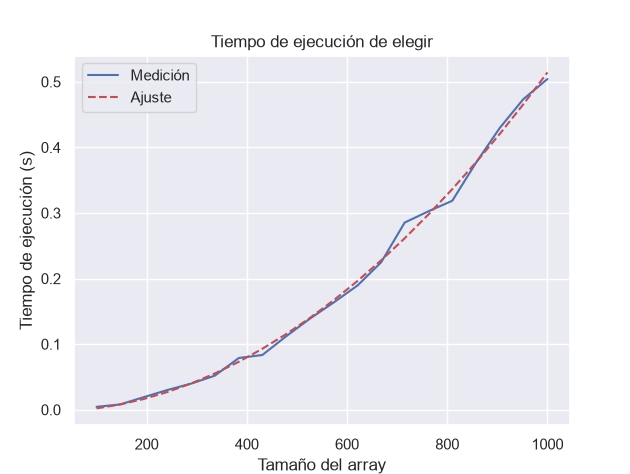
\includegraphics[width=1\textwidth]{img/grafico_analisis.png}
\end{figure}

\subsection{Interpretacion}

Usamos el coeficiente de determinación $R^2$

\begin{itemize}
    \item $R^2 = 1.00$: Ajuste perfecto
    \item $R^2$ mayor $0.98$: Excelente ajuste → Complejidad verificada
    \item $R^2$ mayor $0.95$: Muy buen ajuste → Complejidad muy probable
    \item $R^2$ menor $0.90$: Ajuste pobre → Resultados no concluyentes
\end{itemize}

\subsection{Conclusion}

Con un valor de $R^2 = 0.99$ (mejor que el anterior), concluimos que la complejidad del algoritmo es $O(N^2)$, debido a la alta calidad del ajuste. 
\section{Conclusiones}

Acá irían las conclusiones de todo nuestro trabajo :)
}


\newpage
\end{document}